\documentclass{beamer}
\usetheme{Warsaw}
\usepackage[utf8]{inputenc}


%Information to be included in the title page:
\title{Another wine bar in Paris \\ {Coursera Captsone Project}}
\author{Tom Hohweiller, PhD.}
\date{2021}



\begin{document}

\frame{\titlepage}

\begin{frame}
	\frametitle{Business question}
	\begin{block}{A client problem}
		\begin{itemize}
			\item A client wants to open a wine bar in Paris
			\item In an area with existing restaurants for a dynamic neighbourhood 
			\item But not too many of them
		\end{itemize}
	\end{block}

	\begin{block}{Business understanding}
		\begin{itemize}
			\item Get a location in Paris for a wine-related venue
			\item In an area with already a good medium density of restaurants
		\end{itemize}
	\end{block}
\end{frame}


\begin{frame}
	\frametitle{Methodoly}
	\begin{block}{Planning the study}
		Four steps ahead to find the best location:
		\begin{itemize}
			\item[1.] Extract every venues in each \textit{arrondissement} to have a better view of the business situation
			\item[2.] Study the number of restaurants as well as the number per 1000 residents (for wine bars or shops also)
			\item[3.] After selecting a \textit{arrondissement}, refine the venues and clustering them to identify small area with proeminent restaurants
			\item[4.] Finally, choosing the best area will be our best location in Paris
		\end{itemize}
	\end{block}
\end{frame}


\begin{frame}
	\frametitle{Data - Data requirements}
	\begin{block}{Data needed}		
		Two type of data - for each \textit{arrondissement} and venues
		\begin{itemize}
			\item Coordinates of each \textit{arrondissement} - \textbf{Webscrapping wikipedia webpage}
			\item Venues in Paris for each \textit{arrondissement} - \textbf{Using the Foursquare API}
			\begin{itemize}
				\item Name of the venue
				\item Coordinates
				\item Venue category
				\item Postal code
			\end{itemize}
		\end{itemize}
	\end{block}
\end{frame}

\begin{frame}
	\frametitle{Data - Data understanding and preparation}
	\begin{block}{DataFrame}
		Each dataframes will be usefull, the followed ones will be constructed:
		\begin{itemize}
			\item[1-] DataSet of each \textit{arrondissement}
			\item[2-] DataSet of all the venues (for each \textit{arrondissement})
			\item[3-] DataSet for restaurants and wine bars and shops
			\item[4-] DataSet for the selected \textit{arrondissement}
		\end{itemize}
	\end{block}
\end{frame}


\begin{frame}
	\frametitle{Modeling}
	\begin{block}{Steps to take}		
		\begin{itemize}
			\item[1.] Extract every venues in each \textit{arrondissement} to have a better view of the business situation
			\item[2.] Study the number of restaurants as well as the number per 1000 residents (for wine bars or shops also)
			\item[3.] After selecting a \textit{arrondissement}, refine the venues and clustering them to identify small area with proeminent restaurants
			\item[4.] Finally, choosing the best area will be our best location in Paris
		\end{itemize}
	\end{block}
\end{frame}


\begin{frame}
	\frametitle{WebScrapping and venues}
	\begin{block}{Step 0}
		Webscrapping wikipedia pages is done using \texttt{beautifulsoup}		
	\end{block}
	\begin{block}{Step 1}
		Calling the Foursquare API make gathering venues information really easy
	\end{block}
	These two step created the following dataframes, with the dataframe of each \textit{arrondissement} (left) and data frame of each venues (right).
	%fffffffffffffffffffffffffffffffffffffffffffffffffffffffffffffffffffffff%
	\begin{figure}[h]
		\centering
		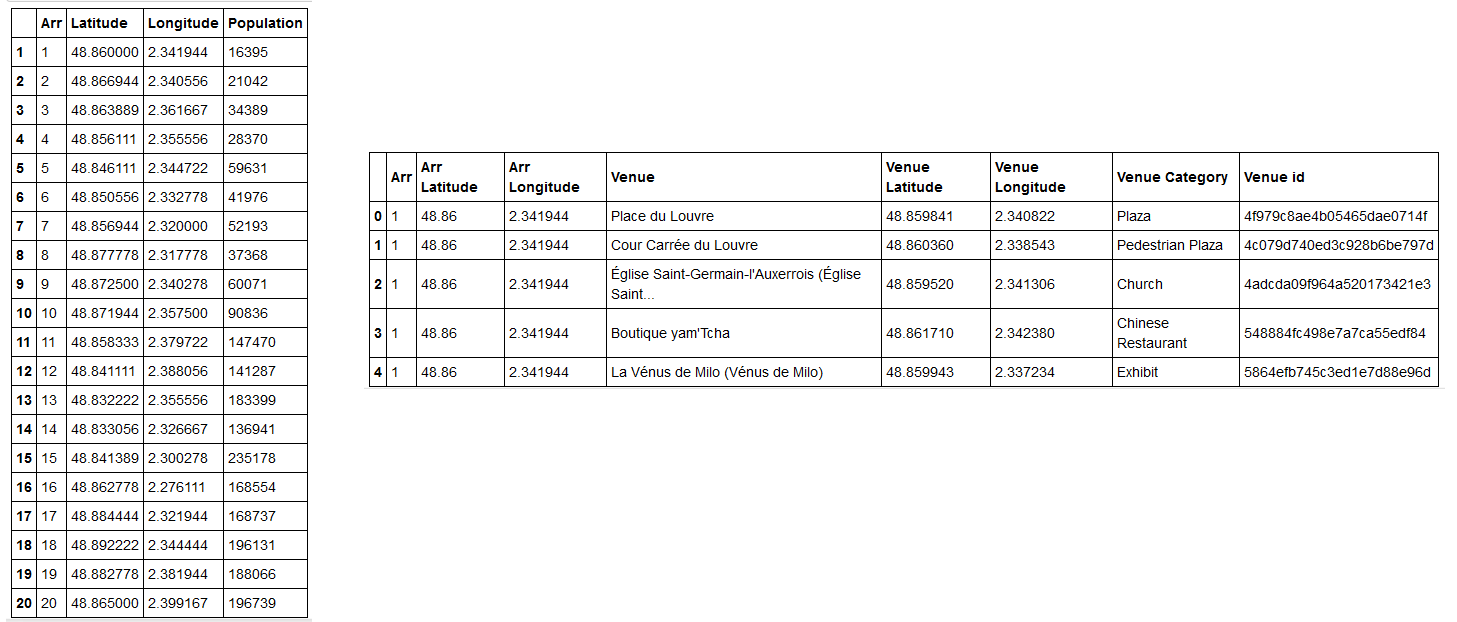
\includegraphics[width=0.75\linewidth,keepaspectratio]{Figures/DataFrameArrVenues}
		\label{DataFrames}
	\end{figure}
	%fffffffffffffffffffffffffffffffffffffffffffffffffffffffffffffffffffffff%	
\end{frame}

\begin{frame}
	\frametitle{Retaurants and wine bars/shops}
	\begin{block}{Step 2}
		Creating a statistic dataframe with the number of restaurants and wine bars/shops, as well a the number of venues per $1000$ residents is easy. Creating bar plots, representing each value for each \textit{arrondissement}
	\end{block}
	%fffffffffffffffffffffffffffffffffffffffffffffffffffffffffffffffffffffff%
	\begin{figure}[h]
		\centering
		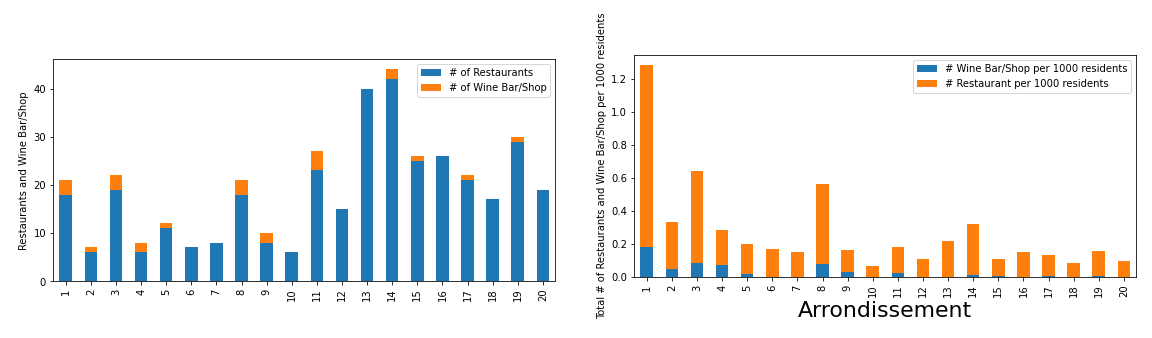
\includegraphics[width=\linewidth,keepaspectratio]{Figures/BarPlots}
		\caption{Bar plots of the total number of restaurants and wine bars/shops (left). Number of restaurants and wine bars/shops per $1000$ residents (right).}
		\label{BarPlots}
	\end{figure}
	%fffffffffffffffffffffffffffffffffffffffffffffffffffffffffffffffffffffff%	
\end{frame}

\begin{frame}
	\frametitle{Best \textit{arrondissement}}
	\begin{block}{Step 3}
		\begin{itemize}
			\item Taking into account the fact that the client wants a area with existing restaurant (but not too many). The \textbf{third \textit{arrondissement}} will be chosen. 
			\item However, take surrounded \textit{arrondissement} is a good solution for broader research
			\item Looking at the following \textit{arrondissement}: $1$st, $2$nd, $3$rd, $4$th, $10$th and $11$th
		\end{itemize}
	\end{block}	
	Creating this dataframe, for all venues in the third \textit{arrondissement}
	%fffffffffffffffffffffffffffffffffffffffffffffffffffffffffffffffffffffff%
	\begin{figure}[h]
		\centering
		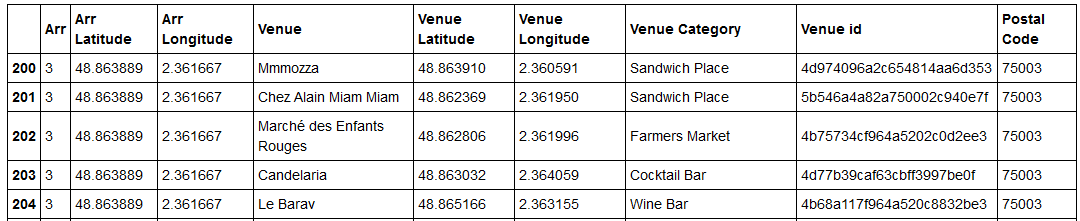
\includegraphics[width=\linewidth,keepaspectratio]{Figures/DataFraleThird}
		\caption{Dataframe of the third \textit{arrondissement} with additional information.}
		\label{DataFramesThird}
	\end{figure}
	%fffffffffffffffffffffffffffffffffffffffffffffffffffffffffffffffffffffff%	
\end{frame}

\begin{frame}
	\frametitle{Best \textit{arrondissement}}
	Venues in these areas are depicted in the following map
	%fffffffffffffffffffffffffffffffffffffffffffffffffffffffffffffffffffffff%
	\begin{figure}[h!]
		\centering
		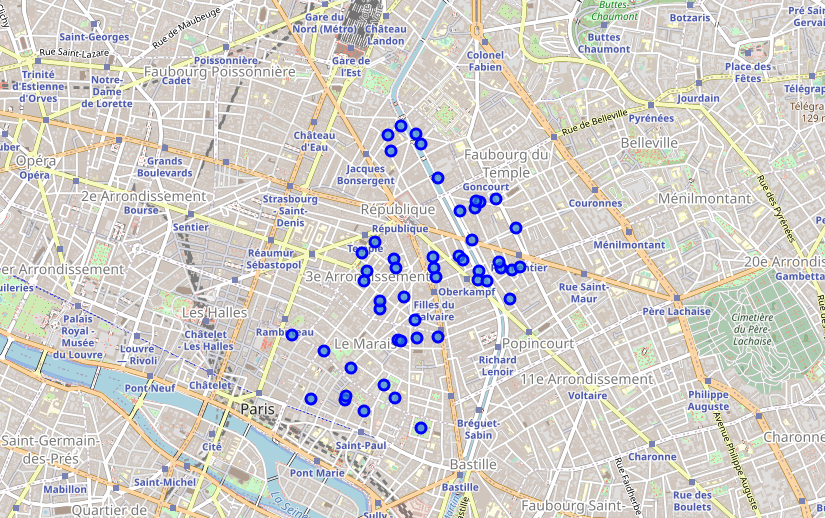
\includegraphics[width=0.80\linewidth,keepaspectratio]{Figures/FoliumUnclustered}
		\caption{Spatial repartition of the venues of the third \texttt{arrondissement} and around.}
		\label{FoliumMap}
	\end{figure}
	%fffffffffffffffffffffffffffffffffffffffffffffffffffffffffffffffffffffff%
\end{frame}


\begin{frame}
	\frametitle{Best \textit{arrondissement}}
	\begin{block}{Step 3.5}
		From the previous map, four area can be found. Using \textit{k-means}, they can be identify
	\end{block}
	%fffffffffffffffffffffffffffffffffffffffffffffffffffffffffffffffffffffff%
	\begin{figure}[h!]
	\centering
	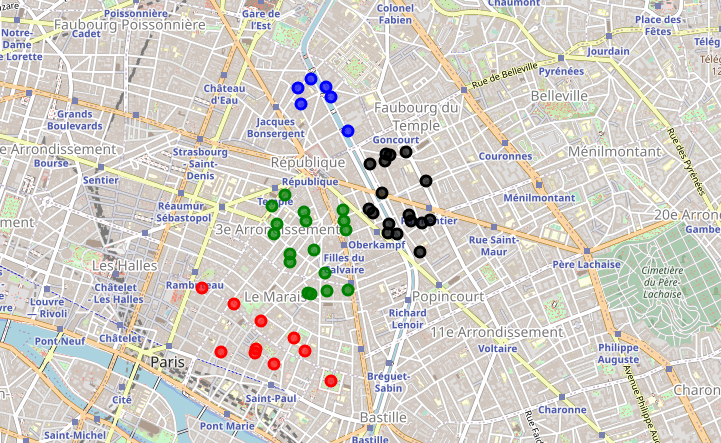
\includegraphics[width=0.60\linewidth,keepaspectratio]{Figures/FoliumClustered}
	\caption{Spatial repartition of the venues of the third \texttt{arrondissement} and around - color coded with respect with cluster label.}
	\label{FoliumMapColored}
	\end{figure}
	%fffffffffffffffffffffffffffffffffffffffffffffffffffffffffffffffffffffff%
\end{frame}

\begin{frame}
	\frametitle{Best area}
	\begin{block}{Step 4}
		From these clusters, the top five venues category can be extracted. Which are the following:
		%fffffffffffffffffffffffffffffffffffffffffffffffffffffffffffffffffffffff%
		\begin{figure}[h!]
			\centering
			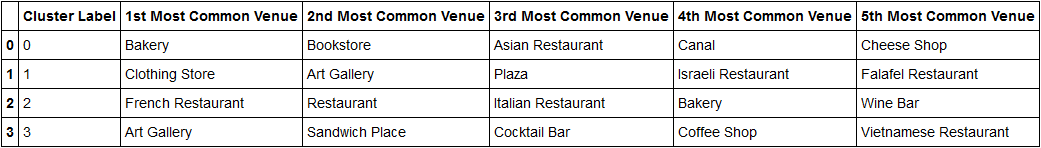
\includegraphics[width=\linewidth,keepaspectratio]{Figures/TopFive}
			\caption{Top $5$ venues category for each clusters.}
			\label{ClustersVenueCat}
		\end{figure}
		%fffffffffffffffffffffffffffffffffffffffffffffffffffffffffffffffffffffff%
		Selecting the cluster label $2$ was done:
		\begin{itemize}
			\item Existing restaurants
			\item Other clusters have day-related venues
			\item Bonus point: close to the Republic place in Paris (lot of people)
		\end{itemize}
	\end{block}
\end{frame}

\begin{frame}
	\frametitle{Best area}
	Finally, the best location would be in the following circle:
	%fffffffffffffffffffffffffffffffffffffffffffffffffffffffffffffffffffffff%
	\begin{figure}[h]
		\centering
		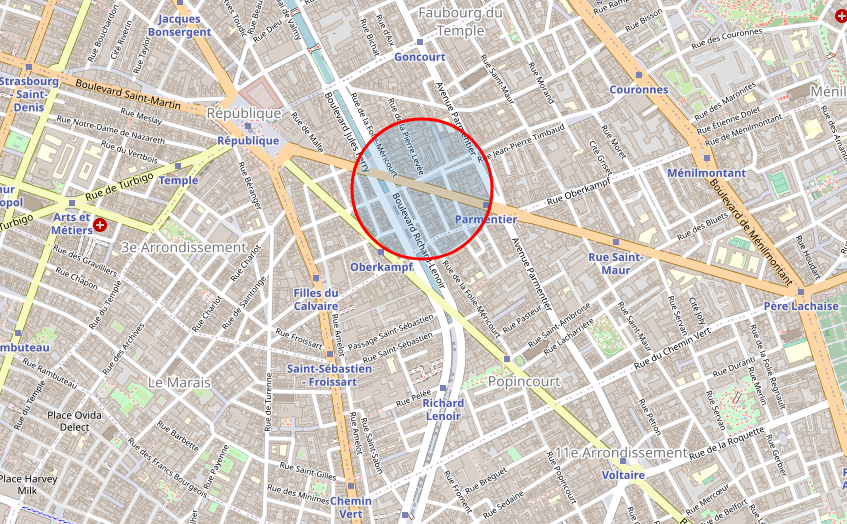
\includegraphics[width=0.8\linewidth,keepaspectratio]{Figures/FoliumFinal}
		\caption{Best location for a wine bar/shop in Paris.}
		\label{FinalLocation}
	\end{figure}
	%fffffffffffffffffffffffffffffffffffffffffffffffffffffffffffffffffffffff%
\end{frame}

\begin{frame}
	\frametitle{Conclusion}
	\begin{itemize}
		\item This study was conducted using several techniques:
		\begin{itemize}
			\item webscrapping
			\item getting information using API
			\item clustering
		\end{itemize}
	\item It was successful at deciding to find the best location for opening a wine bar/shop
	\end{itemize}
\end{frame}


\begin{frame}
	\begin{center}
		\Huge{Thank you for your reading! \\ Hope it was pleasant \\ Have a nice day!}
	\end{center}
\end{frame}

\end{document}